%!TEX root = skripsi.tex
%-----------------------------------------------------------------------------%
\chapter{\babDua}
This chapter focuses on literature study on three aspects including language models, deep learning, and semantic role labeling. In language model section, Part-of-Speech tag (POS tag) and word embedding are described. Deep learning section focuses on the architecture widely used for sequence labeling problem. Finally, we explain semantic role labeling in the last section, including the semantic roles definition, annotation corpus, problem definitions, common features, and the historical perspectives.
%-----------------------------------------------------------------------------%
%-----------------------------------------------------------------------------%
\section{Language Models}
This section explains the language models usually used in Natural Language Processing (NLP) applications. We first describe the traditional yet important language model, Part-of-Speech Tag (POS Tag), followed by word embedding that is often used in recent NLP application with deep learning.

\subsection{Part-of-Speech Tag (POS Tag)}

\subsection{Word Embedding}
Word representation is an important feature when one wants to build deep learning model for NLP tasks. The idea is to convert words into vectors. There are two approaches for this vector representation, which are traditional and word embedding approach. Traditional approach uses one-hot vectors for the representation, meanwhile word embedding approach uses real values vectors that contain information about the words.

In the traditional approach, the vectors are retrieved based on the index of the word found in the dictionary. The dictionary consists of the word and its index. Suppose that we have four words: I, eat, chicken, beef. Each of these words has their own index, with I:0, eat:1, chicken:2, beef:3. These indices will represent the one-hot vectors for the words. For instance, word with index 0 has a one-hot vector [1 0 0 0], word with index 1 has a one-hot vector [0 1 0 0], and so on. The length of the vector is determined by the size of our dictionary. In this case, the size of our dictionary is 4, hence the length of the vector is also 4. 

However, this representation has two drawbacks. First, it hardly depends on the dictionary. If the dictionary does not have the desired word, then it could not represent the word into vector. If we want the dictionary to cover all the words, the size of the dictionary will be extremely huge. Second, the vector representation is sparse. Since we just give the index to the all the words based on the dictionary, it does not really represent an important information from the words. The word ‘hotel’ and ‘hostel’, though have similar context, could be represented by two far indices, say 1 and 100. 

Word embedding aims to address the second issue. Word embedding converts similar words with similar vectors. From the previous example, the word hotel and hostel will have vectors that are close to each other. Hence, the vector representations are dense. Unfortunately, it still could not solve the first drawback that out-of-vocab words could not be represented as vectors.

There has been a lot of research on word embedding (Mikolov et al, 20xx) (Mikolov et al, 20xx) (Mikolov et al, 20xx). In this section, we will explain word embedding architectures proposed by Mikolov, called as Word2Vec. Word2Vec uses unsupervised approach so that we only need a lot of unlabeled data for building word embedding model. Word2Vec has two architectures, which are Context Bags of Words (CBOW) and Skipgram. Fig XX shows the difference between CBOW and Skipgram architectures. In CBOW, the model learns to predict a word based on its neighbouring words.	 In contrast, Skipgram aims to predict the neighbouring words of a word. 

(GAMBAR CBOW DAN SKIPGRAM)

Both architectures mainly aims to build language model. For word embedding model, we do not need the whole architecture model after we finish training the model. Instead, we only need to extract the weight matrix W when the model converts the word index into vector. This weight matrix W is our word embedding model that we use to represent our input words.

\section{Deep Learning}

\subsection{Recurrent Neural Networks}
Recurrent Neural Networks, shortened as RNN, is part of neural network family for processing sequential data. It is thus perfect for modeling the sequence labeling problem. Suppose that we have sequence of inputs, RNN will take each input in a time step t to process it in a function. Figure XX shows a general RNN.

(GAMBAR SEDERHANA RNN)

The left picture illustrates the folded RNN model applied to all time steps. Note that the black rectangle represents one time step delay, meaning that that input is coming from the output of the previous time step. 

The right picture shows the unfolded RNN that is more intuitive since it visualizes the time steps. There are three layers in every time step t, which are input, hidden, and output layers, denoted as x, h, and o respectively. The input layer is for the input representations. In the hidden layer, it contains information from the input layer as well as those coming from hidden layers in the previous time steps. The output layer consists of the output of the model. These three layers are in a form of vectors. In every time step t, RNN has input layer x(t) E R A, hidden layer h(t) E R H, and output layer y(t) E B. The values of A, H, and B, represent the length of the input vector, the number of unit in a hidden layer, and the length of the output vector. There are three parameters that will be trained, which are U, V, and W. These parameters are the weight matrices for connecting two layers. U E R HxA connects input with hidden (input-hidden), W E R HxH  connects hidden with the previous hidden (hidden-hidden) and V E R BxH connects hidden with ouput (hidden-ouput). These parameters are shared across time steps. 

Every input layer x(t) is mapped into output layer o(t) in every time step t. In the middle of the process, it calculates the hidden layer h(t) from two layers, x(t) and h(t-1). The output layer o(t) then is retrieved by performing a function to the hidden layer h(t). The general equations for RNN is presented as follows:
•	h(t) = f1(U. x(t) + W . h(t-1) + b)
•	o(t) = f2(V. h(t) + c)
•	Where h(0) = f1(U . x(0))

Note that there are two additional parameters to train, which are the bias vectors b and c. In the first equation, the input x(t) and h(t-1) is weighted by matrices U and W respectively, added by a bias vector b. The result is then inserted to an activation function f1 in order to produce hidden layer h(t). In the second equation, h(t) is multiplied by the weight matrix V and added by a bias vector c, before being processed by the activation function f2 to produce o(t). The examples of activation function f1 and f2 are tanh and softmax.

Based on this illustration, there are two main characteristics of RNN:

1. It has a cycle in the graph for every time step. Hidden layer h(t) will be one of the inputs for forming h(t+1).

2. It has shared parameters across time steps. 

Fig XX illustrates a more complete RNN model on how it is being trained.

(GAMBAR BAGAIMANA RNN DI TRAIN)

The goal of training the model is to find the estimated values of parameters W, U, V, b, and c which produce outputs o(t) as close as the expected outputs y(t) in the training data. 

The loss function L acts as the measure the difference between the predicted output o(t) and the expected output y(t) in every time step t. The more little the difference, the better the model. The machine thus has to minimize the result of loss function as small as possible. The parameters W, U, V, b, and c are unknown in the beginning. At first, these parameters are initiated randomly.For every iteration (called as epoch), the machine aims to learn the best values for each parameters.

The way to do so is by computing the gradient for each iteration. The idea behind computing the gradient values is to show us which parameter setting that brings us into smaller loss function result. By having this information, the machine then sets the better values for each parameter in the next iteration in order to reduce the loss function. From one iteration into another, the machine will find better parameter values to minimize the loss function. The learning method based on the gradient information is called optimization algorithm such as Stochastic Gradient Descent (), Adam (Kingma and Ba, 2014), and RMSProp (Hinton, 2012)

\subsection{Long Short-Term Memories}
There is an issue in traditional RNN that our networks should overcome, it is called vanishing and exploding gradient problem. The RNN architecture repeatedly uses same parameters for each time steps. Suppose that we use W as the parameter used for each time step between the hidden units. After t time steps, the matrix would be multiplied t times, hence it is the same as multiplying the hidden units with Wt. Assuming that W has an eigendecomposition W = X diag(lambda) X-1, Wt is equal to:

Wt = (X diag(lambda) X-1)t = (X diag(lambda)t X-1)

The eigenvalues lambda in diag(lambda) will either vanish if they are less than 1 in magnitude or explode if they are greater than 1 in magnitude. The gradient counted in each time step is aligned with the eigenvalues. Hence, the gradient may also vanish or explode. This is what we called as vanishing and exploding gradient problem. When the gradient vanishes, it is hard for the machine to find the direction to reduce the cost function. In the case of exploding gradient, the learning algorithm will become unstable.

To address this issue, there are solutions proposed such as leaky units (Mozer, 1992), simulated annealing and discrete error propagation (Bengio et al., 1994), time delays (Lang et al., 1990), and hierarchical sequence compression (Schmidhuber et al., 2007). Among these approach, one of the most robust solutions is called Long Short Term Memories (LSTM) (Hochreiter et. al., 1997). 

The modification used in LSTM to address the issue is by using gates. It is basically RNN, but the nonlinear units in the hidden layer is replaced by the memory blocks. Fig XX shows the difference between RNN and LSTM for the hidden layer. One nonlinear unit tanh in RNN is replaced by a more complex memory blocks in LSTM. Besides the hidden layer h(t), LSTM also has m(t) which is called memory cells.  The idea of LSTM is to learn when to forget or remember the memory from previous time steps through multiplicative gates. It thus prevents the vanishing and exploding gradient problem. For example, if the input gate is closed, then the memory will be unchanged.

(GAMBAR ONE BLOCK MEMORY IN LSTM)

Fig XX illustrates a one block memory in LSTM. There are three main gates which are forget gate, input gate, and output gate. These gates are responsible to determine whether an information is added, kept, or deleted in a cell. Each gate has sigmoid layer and element-wise operations. The sigmoid layer converts the input into a probability between 0 and 1. This probability describes the gate behavior towards the input, whether to accept it (probability close to 1) or not (probability close to 0). 

The equations of the sigmoid layers for each of the gates are explained as follows:

1. Forget Gate

This gate is responsible to determine how much the information from the past should be kept in the memory. The equation of sigmoid layer in forget gate is:

At = sigmoid(WAX X + WAH . h t– 1 + WAM . m t-1)

2. Input Gate

This gate is responsible to determine how much the current information x(t) should be kept in the memory. The equation of sigmoid layer in input gate is:

Bt = sigmoid(WAX X + WAH . h t– 1 + WAM . m t-1)

3. Output Gate

This gate is responsible to determine the output of a time step based on current cell state. The equation of sigmoid layer in output gate is:

Yt = sigmoid(WAX X + WAH . h t– 1 + WAM . m t-1)

In every time step t, the equation for computing cell state m(t) and hidden layer h(t) is presented below:

Mt = At ( x) mt-1 + Bt ( X ) . tanh (Wxmx Xt + Whm. H t-1)
Ht = Yt (x) tanh(mt)


\section{Semantic Role Labeling}
Semantic role labeling (SRL) is a task in Natural Language Processing to assign semantic roles for each argument for each predicate in given input sentence. In this sub-chapter, the definition of semantic roles will be explained. This sub-chapter then explains the most commonly used annotation corpus for SRL. In the end, the details on semantic role labeling task is described.

\subsection{Semantic Roles}
Semantic roles are the representations that express the abstract role of that arguments of a predicate can take in the event (Jurafsky, 2015). When it comes to understanding natural language, one would want to understand the events and their participants of a given input sentence. In this case, the events refer to the predicate and the participants refer to the argument. The example below illustrates the connection between a predicate and its arguments.
Andy         eats      fried chicken
Argument   Predicate    Argument
In this example, eat is the predicate with Andy and fried chicken as its argument. With this point of view, the predicate can be seen as the center of the sentence, followed by the arguments that depend on it.

Knowing the predicate and its arguments is not enough to understand the sentence since the roles of the arguments towards the predicate are unknown. In the previous example, it would be more meaningful to differentiate that Andy is the Eater and fried chicken is the EatenThing. Eater and thing eaten are the examples of semantic roles for the predicate eat. These semantic roles could be used to identify the roles of the arguments regardless its position in the sentence. The previous example could be represented with 2 ways:
Andy         eats      fried chicken
Eater      Predicate      EatenThing
The fried chicken   is eaten    by Andy
EatenThing          Predicate      Eater
Both sentences represent the role of Andy and fried chicken as eater and thing eaten respectively, regardless of their position in the sentence as a subject or object.

There are many ways to define such semantic roles. From the examples above, the semantic roles are very specific for its predicate, known as deep roles (Jurafsky, 2015). Eater and ThingEaten are semantic roles for the predicate eat, Kicker and KickedThing are semantic roles for the predicate kick, and so on. In order to further knowing more about the semantics of these arguments, these semantic roles could be generalized into more abstract roles. Eater and Kicker have something in common: they are volitional actors having direct causal responsibility for the predicate. For this reason, thematic roles are introduced as a set of semantic roles designed to capture semantic commonality between Eater and Kicker (Jurafsky, 2015). With this in mind, Kicker and Eater can be represented as AGENT, which represents the abstract concept that is a volitional causer of an event (or predicate). On the other hand, EatenThing and KickedThing both represent the direct objects that are affected by the event. The semantic role for EatenThing and KickedThing is THEME.

Table x shows the thematic roles often used across computational papers (Jurafsky, 2015).

(TABLE CONTOH SEMANTIC ROLES)


\subsection{Annotation Corpus}
There are available annotated corpus for SRL consists of sentences labeled with semantic roles. Researchers are using these annotated corpus for building supervised machine learning model for SRL. The two most commonly used annotation corpus for SRL are Proposition Bank and FrameNet.

\subsubsection{Proposition Bank}
Proposition Bank, shortened as PropBank, is a corpus in which sentences are annotated with semantic roles. PropBank corpus is available for English, Chinese, .., ..., ... The main approach used for its semantic roles grouping is based on proto-roles and verb-specific semantic roles. Every verb sense has its set of semantic roles with argument numbers rather than names, for example: Arg0, Arg1. Arg2, etc. Generally, Arg0 represents PROTO-AGENT while Arg1 represents PROTO-PATIENT. Other argument number representations may vary based on each verb sense.

The PropBank entries are called frame files. One example of the frame files for one sense of verb eat is presented below.

Frame File:
Eat.01
Arg0: Eater
Arg1: Things Eaten
Arg2: Instrument used

Example:
Ex1: [Arg0 Andy] eats [Arg1 fried chicken] [Arg2 with spoon]
Ex2: [Arg1 That fried chicken] is eaten by [Arg0 Andy] [Arg2 with spoon]

For verb sense Eat.01, Arg0 acts as the Eater (PROTO-AGENT), and Arg1 represents the Things Eaten (PROTO-PATIENT). As we can see from the example above, we can infer the commonality between examples Ex1 and Ex2 regardless its structure, be it in a passive or active voice. In both examples, Andy is the Eater and fried chicken is the Things Eaten. In this frame file, there is also another argument, Arg2, that represents the instrument used by the Eater. In example Ex1 and Ex2, the instrument is spoon.

Other non-numbered arguments are available in PropBank, the so-called ArgMs, representing modifiers that could be used across frame files. Some examples of ArgMS include:

TMP: When?
LOC: Where?
DIR: Where to/from?

The next annotation corpus is called FrameNet which has different approach on how to group set of semantic roles. Instead of using verb-specific, it uses frame-specific grouping.

\subsubsection{FrameNet}
FrameNet is an annotation corpus for semantic roles that are specific to a frame. In PropBank, the semantic roles are defined based on each sense of a verb. In contrast, a frame in FrameNet could include more than one predicate (verbs or nouns) that have the same background context. Each frame consists of two elements: 1. A set of semantic roles related to this frame, and 2. A set of predicates using the respective semantic roles.

One example is a frame called change position on a scale defined as:
This frame consists of words that indicate the change of an Item’s position 
on a scale (the Attribute)from a starting point (Initial value) 
to an end point (Final value)
The set of semantic roles for a frame is divided into two roles: Core roles and Non-Core Roles. Core Roles are specific to a frame while Non-Core Roles are more general across frames (like ArgMs in PropBank). The set of semantic roles of the frame change position on a scale is explained as bellow:

Core Roles
ITEM: The entity that has a position on the scale.
ATTRIBUTE: The ATTRIBUTE is a scalar property that the ITEM possesses
DIFFERENCE: The distance by which an ITEM changes its position on the scale. FINAL STATE: A description that presents the ITEM’s state after the change in the ATTRIBUTE’s value as an independent predication.
FINAL VALUE: The position on the scale where the ITEM ends up. 
INITIAL STATE: A description that presents the ITEM’s state before the change in the ATTRIBUTE’s value as an independent predication.
INITIAL VALUE:The initial position on the scale from which the ITEM moves away. 
VALUE RANGE: A portion of the scale, typically identified by its end points, along which the values of the ATTRIBUTE fluctuate. 
Non-Core Roles
DURATION SPEED GROUP
The length of time over which the change takes place.
The rate of change of the VALUE.

The possible predicates of the frame change position on a scale are:
VERBS: dwindle move advance edge climb decline dip double drop reach
decrease fluctuate rise diminish gain
soar mushroom swell
explode plummet swing fall triple tumble rocket grow shift slide increase skyrocket decline jump
escalation shift explosion tumble fall fluctuation ADVERBS: gain increasingly NOUNS: hike 
decrease ris
The example of semantic roles of the frame change position on a scale could be seen as follows:

(22.20) [ITEM Oil] rose [ATTRIBUTE in price] [DIFFERENCE by 2%]. 

(22.21) [ITEM It] has increased [FINAL STATE to having them 1 day a month]. 

(22.22) [ITEM Microsoft shares] fell [FINAL VALUE to 7 5/8]. 

(22.23) [ITEM Colon cancer incidence] fell [DIFFERENCE by 50%] [GROUP among men]

(22.24) a steady increase [INITIAL VALUE from 9.5] [FINAL VALUE to 14.3] [ITEM in dividends]

(22.25) a [DIFFERENCE 5%] [ITEM dividend] increase... 

As we can see from the examples above, rose, fell, and increase have the same set of semantic roles under the frame change position on a scale. Instead of defining the semantic roles for each verb sense one by one, FrameNet groups predicates (not limited to verbs) that have the same semantic roles as one frame.

\subsection{Problem Definitions}
Semantic Role Labeling (SRL) is one of Natural Language Processing task which aims to automatically assign semantic roles for each constituent (argument) for each predicate in a sentence (Jurafsky, 20XX). Current approach to solve this task is by using supervised machine learning. Given a labeled data, the machine learns from it and builds a generalization model. Researches often used PropBank or FrameNet corpus as the sources of annotated data. In this section, we describe the approaches to define the problem of SRL task, followed by the common features used for building supervised model for SRL.

There are two ways to see SRL problem, either as Classification or Sequence Labeling problem (Someone, 20XX). Classification approach assigns semantic roles for each word independently. Meanwhile, Sequence Labeling approach traverses from assigning semantic role for the first word until the last one in a sentence sequentially. In Sequence Labeing, the next label (semantic role) prediction of time step t is dependent to labels predicted on previous time steps (1..t-1). The differences of these two approaches to solve SRL task are visualized in Fig X.

[Fig X. The visualizations of the differences of Classification approach and Sequence Labeling approach]

The general algorithm for SRL based on Classification approach is explained as follows.
Function SEMANTICROLELABEL(words) returns labeled tree
Parse <- Parse(words)
For each predicate in parse do
For each node in parse do
Featurevector <- EXTRACTFEATURES(node, predicate, parse)
CLASSIFYNODE(node, featurevector, parse)

Explanation on SRL based on Classification approach:
•	Parsing input sentence into a parse tree
•	Traverse the parse tree to find all the predicates
•	For each predicate, traverse each node (word) in a parse tree to
o	Extract features
o	Classify the node based on features extracted. 
	1-of-N classifier is trained here to predict the semantic role for each node (word) in a parse tree.
	N is the number of possible semantic roles added with 1 Other role for word that has no semantic roles.

The classification algorithms that have been used to train 1-of-N classifier include logistic regression (Someone, 20xx) and SVM (Someone, 20xx).

[Penjelasan untuk algoritme Sequence Labeling approach]

\subsection{Common Features for SRL}
•	The first set of features for SRL is proposed by Gildea and Jurafsky (2000).
o	They are the first ones who used supervised machine learning approach to solve SRL. 
o	Over the years, many research proposed new set of features to improve the result, but they still used the basic features proposed by Gildea and Jurafsky (2000).
o	Common features used for solving SRL task are:
	The predicate. 
•	Usually in a form of verb.
	The phrase type of the constituent.
•	NP, PP, etc
	The headword of the constituent.
•	The black bird. Headword: bird.
	The headword part of speech of the constituent. 
•	Example: NNP.
	The path of the parse tree from constituent to predicate. 
•	This is to represent the grammatical relationships between the constituent and the predicate.
•	Example: NP S VP VBD
	The voice of the clause, active or passive.
•	Example: I eat chicken rice (active), Chicken rice is eaten by me (passive).
	The binary linear position of the constituent from the predicate.
•	Could be before or after the predicate.
	The subcategorization of the predicate
•	Set of arguments that appear in the verb phrase VP.
•	Example: NP and PP in ‘VP -> VBD NP PP’
	The named entity type of the constituent
•	Example: Organization, Person, Location, ..
	The first and last words of the constituent.
o	There are also other additional features that could be used for SRL.
	Sets of n-grams inside the constituent.
	Using dependency parser instead of syntactic parser for extracting features.

\subsection{Historical Perspectives}
SRL can be seen as either a classification or sequence labeling problem. The earlier research on SRL was conducted with the classification approach, meaning that each argument is being predicted independently from the others. Those research focused on how to extract meaningful features out of syntactic parsers~\cite{gildea2002automatic, gildea2002necessity, pradhan2005semantic}, such as the path to predicate and constituent type. This syntactic information plays a pivotal role in solving SRL problem~\cite{punyakanok2008importance} as it addresses SLR's long distance dependency~\cite{zhou2015end}. Thus, traditional SRL system heavily depends on the quality of the parsers. The analysis done by Pradhan et al. shows that most errors of the SRL system were caused by the parser's error \cite{pradhan2005semantic}. In addition, those parsers are costly to build, since it needs linguistic experts to annotate the data. If we want to create an SRL system on another language, one should build a new parser all over again for it.~\cite{zhou2015end}.

In order to minimize the number of hand-crafted features, Collobert et al. utilized deep learning for solving NLP tasks including Part-of-Speech Tagging (POS), Chunking (CHUNK), Named Entity Recognition (NER), and Semantic Role Labeling (SRL) with classification approach~\cite{collobert2011natural}. The research aims to prevent using any task-specific feature in order to achieve state-of-the-art performance. The word embedding is used as the main feature across tasks, combined with Convolutional Neural Networks (CNN) architecture to train the model. They achieve promising results for the POS Tagging and Chunking, while for SRL features from the parsers are still needed to achieve competitive results.

Different from the previous works, Zhou et al. view SRL as a sequence labeling problem in which the arguments are labeled sequentially instead of independently~\cite{zhou2015end}. They proposed an end-to-end learning of SRL using Deep Bi-Directional Long Short-Term Memories (DB-LSTM), with word embedding as the main feature. Their analysis suggests that the DB-LSTM model implicitly extracts the syntactic information over the sentences and thus, syntactic parser is not needed. The research result outperforms the previous state-of-the-art traditional SLR systems as it achieves F1 score of 81,07\%. The research also shows that the performance of the sequence labeling approach using DB-LSTM is better than the classification approach using CNN, since the DB-LSTM can extract syntactic information implicitly.

While many of the previous works studied SRL on formal language, our research aims to explore SRL on conversational language, which is still under-resourced. We thus introduce a new set of semantic roles for this language type. Furthermore, we propose a new architecture named Context-Aware Bi-Directional Long Short-Term Memories, designed with attention mechanism in order to capture context information of the sentence at a higher level.

% OR THIS ONE, ELLABORATE BOTH %
Previous research have found useful to use RNN for NLP task Semantic Role Labeling (SRL). Before we discuss about the use of RNN on SRL, we describe the historical perspective of solving SRL with supervised machine learning. We divide the historical perspective based on SRL systems without and with deep learning.

The non-deep learning approach uses specific hand-crafted features for SRL, which mainly depend on syntactic or dependency parser as explained in section 2.XX. It started from Gildea et. Al (2002) who firstly build supervised machine learning model for SRL. The goal of the research was to create the first shallow semantic role parser which is not domain specific, since at that time all the semantic roles research were too domain specific. The features used are extracted from the syntactic tree Collins Parser (XX, 1997), such as Phrase Type, Parse tree path, voice, and head word. Then the predicate of a sentence is also added as a feature. The research used semantic role annotation based on FrameNet. The algorithm used was statistical classifier with backoff approach. The result is 65\% precision and 61\% recall.

Then, Gildea et al (2002) continues the research to quantify the effect of parser accuracy on SRL system’s performance. The research also examines whether a flatter “chunked” representation (which is less costly) of the input can be as effective as syntactic tree parser. The data used is from PropBank dataset, since it is from Wall Street Journal corpus that has a gold-standard syntactic parse trees for the entire dataset from the Penn Treebank Project. The finding shows that the parser accuracy affects the SRL system, since it is seen that the system with gold-standard parse tree impacts directly to build a better SRL system. Hence, the syntactic parser is an integral intermediary model to build a robust SRL system. If the parser is not good, one would not get a good SRL system.

Surdeanu et al (2003) proposed a new set of features for SRL system, such as POS Tag of Head Word, POS Tag of content word, and Named Entity Class of Content Word. They use inductive learning through decision trees C5 for the algorithm.

Xue et al (2004) aims to explore more information extracted from the parse tree in order to propose new set of features crafted to improve SRL. In their research, there are three steps for the model, pruning, argument identification, and argument classification. Pruning filters out constituents that are clearly not semantic arguments to the predicate. Argument identification classifies candidates as either semantic arguments or non arguments. Argument classification then runs a multi-category classifier to classify the constituents with semantic roles. The features proposed for the argument classification are syntactic frame, lexicalized constituent type, lexicalized head word, and the head of Preposition Phrase parent.

Since the source of SRL system errors mostly based on syntactic parser’s error, Pradhan et al (2005) combines features from different syntactic parsers (Charniak parser and Collins Parser). The idea of combining two parser is that they train separate SRL systems for each tree parser. The role output from these two systems is used as additional features in a SRL system using flat syntactic view. They then use SVM classifier to train SRL based on PropBank data.

Aside from using syntactic parse tree like Charniak or Collins parser, one can build SRL system by extracting features from dependency parser. Some of the features extracted are word property, syntactic connection, semantic connection, and dependency path.

The drawbacks of using the non-deep learning approach are 1.) building syntactic or dependency parsers is costly, 2.) the SRL system hardly depends on the robustness of the parsers. Building tree parsers is costly because it is language-dependent and it needs experts in each language to create it. When we move to another language, we have to build these parsers for the new language from scratch. Not to mention a new problem arises when such parsers are not robust, hence creating error propagation in our SRL system. The analysis in Pradhan et al., (2005) says that the major source of errors in SRL system comes from the errors of the syntactic parsers from which we extract the features.

To address this issue, Collobert et al. (20XX) firstly introduced the use of deep learning for SRL and other core NLP tasks such as POS Tagging and Chunking. They use Convolutional Neural Network (CNN) with no task-specific features for the system. For example, in non-deep learning approach, we use POS Tagging features for Chunking, and we use both of which as the features for SRL. Instead, the main feature used in this research is word embedding. As explained in the previous section, word embedding model converts words to vectors. The word vectors then are fed into CNN architecture. However, though the model achieved state-of-the-art performances for POS Tagging and Chungking, that is not the case for SRL. For SRL, it is still needed to use features from the tree parser to achieve robust performance.

Zhou et al., (2015) proposed new architecture for the SRL system. Instead of seeing the SRL as a classification problem like the previous research including Collobert’s, Zhou considers SRL as the sequence labeling problem. Hence, the suitable architecture for such problem is Recurrent Neural Networks (RNN). In their research, a more specific RNN architecture is used, which is Long Short Term Memories (LSTM) in order to prevent the vanishing and exploding gradient problem in RNN. They used the deep bi-directional LSTM. The “deep” is for extracting more hidden features and the “bi-directional” is for extracting information from the past and future. On top of the LSTM architecture, they used Conditional Random Field (CRF) for the output layer. For the word representation, they also used word embedding as one of the main features, along with predicate and context predicate. Our research is mainly inspired by this research.

% PUNYA WAHID %
\section{Pengenalan Entitas Kesehatan}\label{aboutmer}
%-----------------------------------------------------------------------------%
% Apa itu MER
Pengenalan Entitas Kesehatan atau disebut juga dengan \textit{Medical Entity Recognition} (\mer) merupakan salah satu cabang dari Pengenalan Entitas Bernama (\textit{Named Entity Recoginition}) atau disingkat NER dengan dokumen sumber berupa teks kesehatan. NER sendiri merupakan suatu sistem/aplikasi yang memanfaatkan teknik pada \textit{Natural Language Processing} dan \textit{Information Extraction} untuk mengenali entitas yang telah dikategorikan sebelumnya seperti nama, lokasi, organisasi, waktu dan sebagainya. Sedangkan pada sistem MER, entitas yang akan dikenali yaitu entitas yang berada pada domain kesehatan seperti nama penyakit (\textit{\disease}), gejala penyakit (\textit{symptom}), obat (\textit{\drug}), langkah penyembuhan (\textit{\treatment}), nama protein, DNA, RNA dan lain sebagainya. Gambar \ref{fig:mer_ilustration} merupakan ilustrasi dari sebuah sistem \mer.

% Contoh tentang MER
\begin{figure}
	\centering
	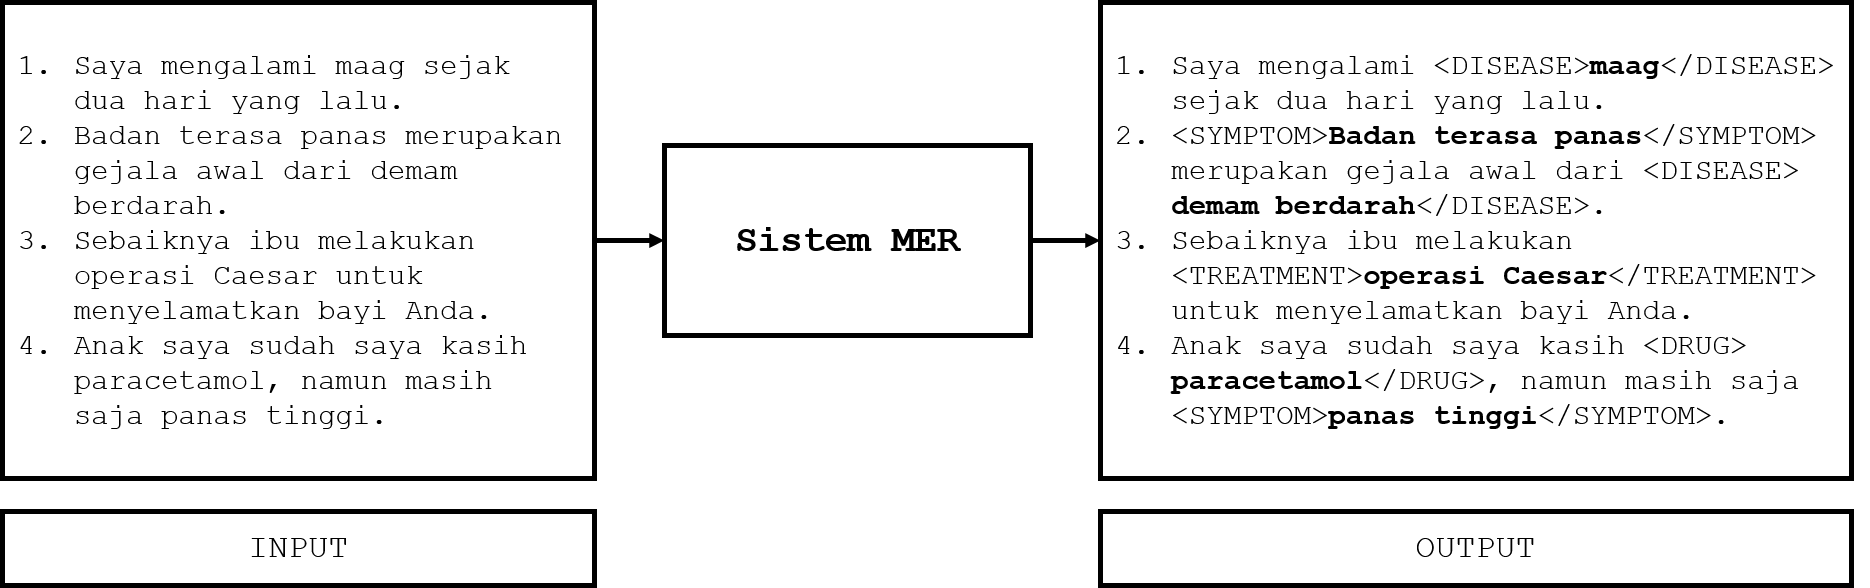
\includegraphics[width=1.0\linewidth]{images/mer_ilustration}
	\caption{Ilustrasi Sistem \mer}
	\label{fig:mer_ilustration}
\end{figure}

Dari ilustrasi di atas, sebuah sistem MER akan diberikan \textit{input} berupa dokumen kesehatan, kemudian sistem diharapkan dapat memberikan \textit{output} berupa dokumen yang sudah diberi label dengan benar. Dokumen kesehatan yang menjadi \textit{input} dapat berupa dokumen formal seperti dokumen suatu rumah sakit atau dokumen non-formal seperti dokumen forum kesehatan \textit{online}.

% Manfaat MER %
Implementasi sistem \mer~dapat memberikan manfaat pada beberapa bidang, seperti pada aplikasi \textit{Question Answering} \citep{abacha2011medical} yang hasil pelabelan dari sistem \mer~dapat mempermudah identifikasi entitas yang ditanyakan. Selain itu, hasil pelabelan sistem \mer~juga dapat dimanfaatkan untuk pembuatan sistem \textit{indexing} dokumen forum sehingga pencarian dokumen kesehatan dapat dilakukan dengan lebih efisien. Sistem \mer~juga dapat digunakan untuk mendukung aplikasi \textit{entity linking} yang memungkinkan seseorang untuk mengetahui hubungan antar entitas \citep{hachey2013evaluating}. Misalnya dengan adanya aplikasi \textit{entity linking}, kita dapat mengetahui obat apabila hanya diberikan \textit{query} nama penyakit dengan \textit{resource} dokumen-dokumen kesehatan yang telah mendapatkan pelabelan dari sistem \mer. Masih banyak manfaat lain dari implementasi sistem \mer~ini.

% Cerita MER Bahasa Inggris %
Sebelumnya \cite{abacha2011medical} telah melakukan penelitian terkait sistem \mer~pada dokumen berbahasa Inggris. Sistem \mer~yang dibuat bertujuan untuk melabeli entitas \textit{treatment}, \textit{problem} dan \textit{test} dengan menggunakan 3 metode, yaitu (i) metode semantik dengan menggunakan \textit{tools} MetaMap (\textit{domain knowledge}), (ii) ekstraksi frasa berdasarkan \textit{chunker} dan klasifikasi dengan SVM (\textit{Support Vector Machine}) dan (iii) gabungan 2 metode sebelumnya dengan menggunakan CRF (\textit{hybrid}). Metode \textit{hybrid} yang dimaksud yaitu dengan menggunakan \textit{tools} CRF sebagai \textit{tools machine learning} yang ditambahkan fitur \textit{domain knowledge}, yaitu fitur semantik yang diekstraksi dengan \textit{tools} MetaMap. Hasil yang terbaik didapatkan dengan menggunakan metode \textit{hybrid} yang menggabungkan 2 metode sebelumnya (\textit{domain knowledge} dan \textit{machine learning}) dan dengan \textit{precision} $ 72.18\% $, \textit{recall} $ 83.78\% $ dan \textit{f-measures} $ 77.55\% $.

Selain penelitian di atas, \cite{mujiono2016new} juga melakukan penelitian terkait \mer~pada dokumen berbahasa Indonesia. Model \mer~yang dikembangkan adalah untuk melabeli entitas \textit{drug} saja. Penelitian tersebut bertujuan untuk mendapatkan representasi data yang berdasarkan karakteristik \textit{training data}. \cite{mujiono2016new} mengusulkan tiga teknik representasi data yang berdasarkan karakteristik distribusi kata dan kemiripan kata dari hasil \textit{training} dari model \textit{word embedding}. Representasi data yang dimasud adalah: (i) semua kalimat diformat sebagai \textit{sequence} token, (ii) semua kalimat di-\textit{generate} menjadi beberapa \textit{sequence}, dan (iii) data direpresentasikan sebagai vektor dengan \textit{tools} \textit{Word Embedding}. Masing-masing representasi kata tersebut dievaluasi dengan masing-masing evaluator, yaitu (i) evaluasi dengan model \textit{neural networks} standar, (ii) evaluasi dengan dua \textit{deep network classifiers}, yaitu DBN (\textit{Deep Belief Networks}), dan SAE (\textit{Stacked Denoising Encoders}) serta (iii) representasi kalimat sebagai vektor \textit{word embedding} yang dievaluasi dengan \textit{recurrent neural networks} yaitu LSTM (\textit{Long Short Term Memory}). Hasil yang didapatkan yaitu kalimat sebagai \textit{sequence} yang dievaluasi dengan LSTM memberikan hasil yang terbaik, yaitu \textit{f-measure} $ 86.45\% $.

% Cerita MER Bahasa Indonesia (Kak Radit, Performa, Tabel) %
Penelitian terkait \mer~pada dokumen berbahasa Indonesia sudah dilakukan sebelumnya oleh \cite{skripsiKakRadit}. Dalam penelitiannya, \cite{skripsiKakRadit} menggunakan CRF (\textit{Conditional Random Fields}) untuk proses pelabelan. Kemudian, pada pekerjaan yang Herwando (2006) lakukan, sebagian besar digunakan untuk mencari fitur-fitur yang memang diskriminatif untuk masalah \mer~yang menghasilkan akurasi terbaik. Entitas yang akan diberi label yaitu nama penyakit (\textit{\disease}), gejala penyakit (\textit{sympton}), obat (\textit{\drug}) dan langkah penyembuhan (\textit{\treatment}). Dokumen yang menjadi \textit{input} penelitian merupakan hasil \textit{crawling} dari  forum kesehatan \textit{online} dari berbagai situs yang berisi tanya jawab. Hasil yang didapatkan yaitu \textit{precision} $ 70.97\% $, \textit{recall} $ 57.83\% $ dan \textit{f-measeure} $ 63.69\% $ dengan fitur \textit{its own word}, frasa, kamus (\textit{symptom}, \textit{disease}, \textit{treatment} dan \textit{drug}), \textit{window feature (previous word)} dan panjang kata.

Selain itu, \cite{suwarningsih2014imner} juga melakukan penelitian terkait \mer~pada dokumen berbahasa Indonesia dengan menggunakan SVM (\textit{Support Vector Machine}), dengan SVM yang digunakan untuk klasifikasi per-kata. Entitas yang akan dikenali yaitu \textit{location}, \textit{facility}, \textit{diagnosis}, \textit{definition} dan \textit{person}. Data yang digunakan sebagai korpus merupakan data dari situs \textit{http://health.detik.com/}, \textit{http://detikhealth.com/} dan \textit{http://health.kompas.com/konsultasi/} dengan total keseluruhan sebanyak 1000 kalimat. Akurasi yang dihasilkan yaitu $ 90\% $ dengan menggunakan fitur \textit{baseline}, \textit{word level (morphology, POS-Tag, dll)} dan fitur dari dalam dokumen tersebut.

\section{Deep Learning}
\textit{Deep Learning}, atau disebut juga \textit{deep structured learning, hierarchical learning,} dan \textit{deep machine learning} merupakan salah satu cabang dalam \textit{machine learning} yang model komputasinya terdiri dari beberapa layer. \textit{Deep learning} mampu mempelajari dan mengekstrak representasi data/fitur secara otomatis pada abtraksi tingkat tinggi \citep{lecun2015deep}. Model tersebut memberikan hasil yang sangat baik dalam penelitan di berbagai bidang seperti \textit{speech recognition}, \textit{object detection}, \textit{sequence labeling} dan lain sebagainya.  

Struktur pembelajaran pada \textit{deep learning} berbentuk hierarki karena termotivasi dari bagaimana neokorteks pada otak maunusia bekerja secara mendalam. Neokorteks tersebut melakukan proses pemelajaran berlayer dan secara otomatis mampu mengketrak fitur dan melakukan abstraksi dari \textit{resource} yang diberikan \citep{bengio2007scaling}. Struktur tersebut terdiri atas \textit{input layer}, \textit{hidden layer} dan \textit{output layer}. \textit{Input layer} memiliki fungsi sebagai tempat masuknya data yang akan dipelajari oleh model. \textit{Hidden layer} melakukan aproksimasi fungsi untuk mendapatkan target dari data \textit{training} yang diberikan. Disebut \textit{hidden layer} karena pada layer ini, \textit{output} tidak bisa kita lihat \citep{Goodfellow-et-al-2016-Book}. \textit{Hidden layer} inilah yang menjadi \textit{key role} dalam \textit{deep learning}. Sedangkan \textit{output layer} merupakan layer untuk mengembalikan target yang diinginkan.

\textit{Deep learning} ini mampu memberikan model yanng memiliki performa sangat baik dalam \textit{supervised learning} \citep{Goodfellow-et-al-2016-Book}. Dengan menambahkan lebih banyak layer dan unit di dalam layer, \textit{deep network} dapat merepresentasikan fungsi dengan kompleksitas yang tinggi. Secara umum, \textit{deep learning} memetakan \textit{input vector} ke \textit{output vector}. Walaupun hal ini mudah dilakukan oleh manusia secar manual, namun untuk \textit{dataset} yang sangat besar, tentu hal ini tidak mungkin dilakukan. Ada banyak macam model \textit{Deep Learning} yang sesuai dengan kebutuhan komputasi, seperti \textit{Deep Belief Network} \citep{hinton2006fast}, \textit{Recurrent Neural Networks} \citep{elman1990finding}, \textit{Long Short Term Memory} \citep{hochreiter1997long}, \textit{Restricted Boltzman Machine} \citep{pennington2014glove} dan lain sebagainya. 

\section{Recurrent Neural Networks}\label{sec:rnns}

\textit{Recurrent neural networks} (RNNs) merupakan merupakan salah satu arsitektur \textit{Deep Learning} yang memiliki koneksi siklik \citep{graves2012neural}. RNNs memiliki \textit{neuron} yang terkoneksi dengan \textit{neuron} lain sehingga membentuk \textit{loop} umpan balik (\cite{haykin2009neural}), tidak seperti \textit{feedforward neural network} (FNNs) dimana aliran informasi hanya berjalan searah. RNNs memungkinkan \iob~yang dihasilkan akan menjadi \ioa~untuk menghasilkan \iob~yang lain. Hal ini menyebabkan perilaku RNNs tidak hanya bergantung pada \ioa~saat ini saja, namun juga bergantung pada \iob~sebelumya. Oleh karena itu, RNNs memiliki kemampuan yang sangat bagus sebagai model dalam permasalahan \textit{sequence data} dibandingkan dengan FNNs. RNNs sendiri memiliki kemampuan yang sangat bagus dalam beberapa \textit{task} terkait \textit{sequence data}, seperti \textit{language model} (\cite{mikolov2010recurrent}) dan \textit{speech recognition} (\cite{graves2013speech}).

Dibandingkan dengan FNNs, RNNs memiliki beberapa kelebihan \citep{mikolov2010recurrent}, yaitu:
\begin{enumerate}
	\item Pada RNNs, kata-kata sebelumnya direpresentasikan dengan \textit{recurrent connections}, sehingga RNNs dapat menyimpan informasi kata sebelumnya dalam jumlah tak hingga. FNNs tidak bisa secara alami memodelkan hubungan kontekstual antara sebuah kata dengan kata-kata pada posisi sebelumnya dan representasi kata sebelumnya berupa konteks dari $ n-1 $ kata. Oleh karena itu, FNNs terbatas dalam penyimpanan informasi kata sebelumnya terbatas seperti pada model \textit{n-gram}.
	\item RNNs dapat melakukan kompresi keseluruhan riwayat kata menjadi ruang dimensi yang lebih kecil, sedangkan FNNs melakukan kompresi/proyeksi hanya dengan sebuah kata saja.
\end{enumerate}

Banyak variasi RNNs yang telah diusulkan oleh beberapa peneliti, seperti Elman \textit{networks} \citep{elman1990finding}, Jordan \textit{networks} \citep{jordan1986attractor}, \textit{time delay neural networks} \citep{lang1990time} dll. Gambar berikut merupakan contoh  dari RNNs secara umum

\begin{figure}
	\centering
	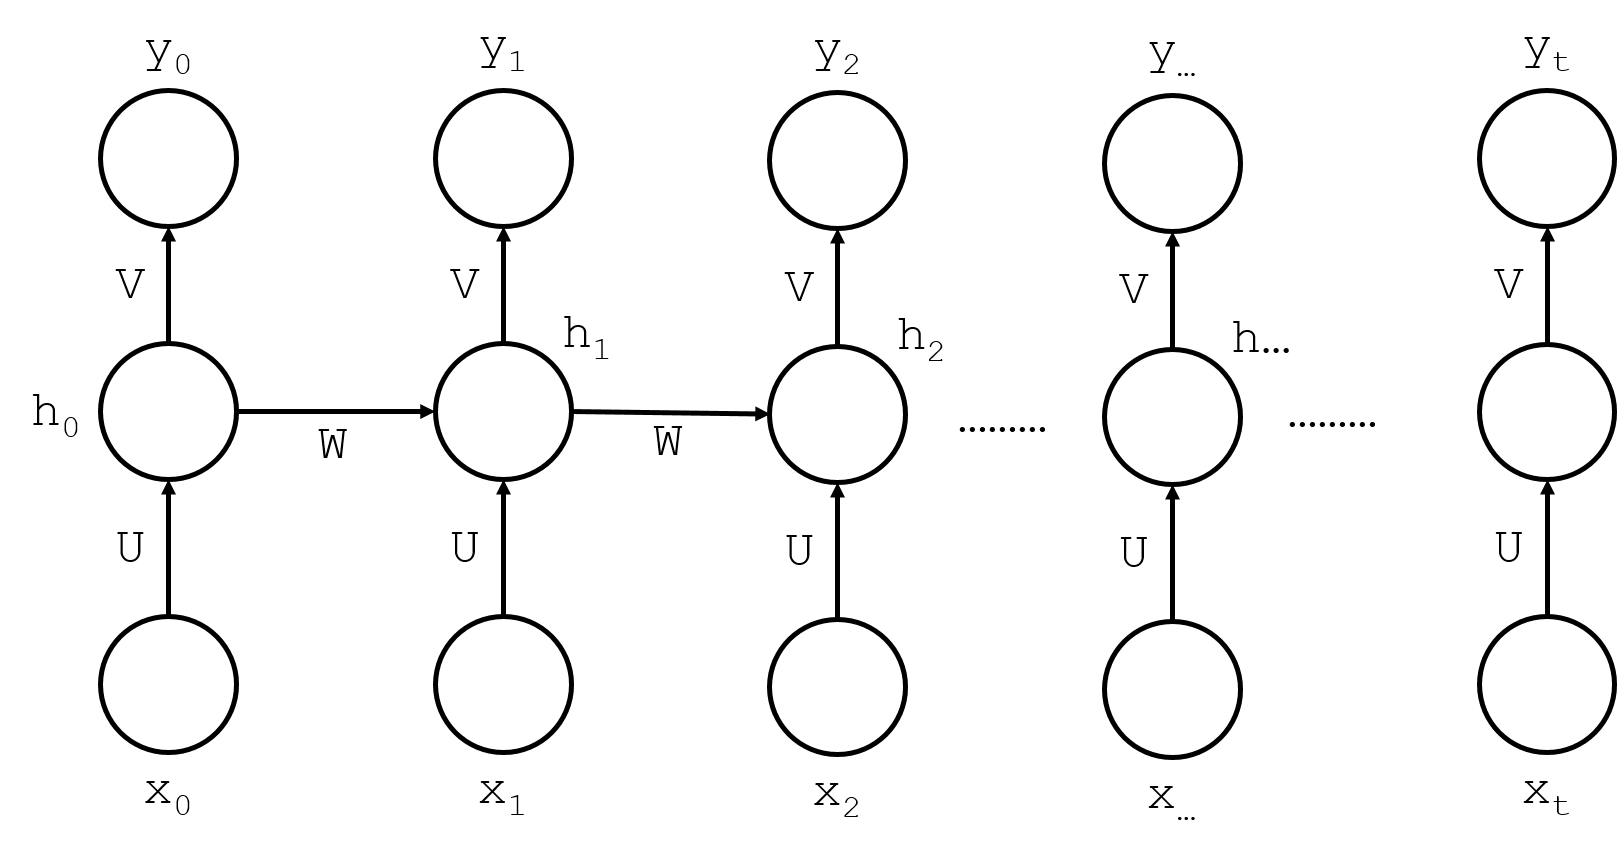
\includegraphics[width=0.80\linewidth]{images/simple_rnn}
	\caption{\textit{Recurrent Neural Networks} sederhana}
	\label{fig:simple_rnn}
\end{figure}

Dari gambar \ref{fig:simple_rnn}, sebuah jaringan pada RNNs memiliki 3 layer pada setiap \textit{timestep}, yaitu \textit{input layer}, \textit{hidden layer} dan \textit{output layer}. \textit{Input layer} merupakan layer sebagai tempat masuk \textit{resource}. Di dalam \textit{hidden layer} tersebut terdapat beberapa unit untuk menyimpan informasi dari \textit{timestep} sebelumnya. Sedangkan pada \textit{output layer} merupakan layer yang memberikan \textit{output} dari model. Pada setiap \textit{timestep} $ t $, RNNs di atas memiliki sebuah \textit{input layer} $ \vec{x(t)} \in {\rm I\!R^{N}} $, \textit{hidden layer} $ \vec{h(t)} \in {\rm I\!R^{H}} $, dan \textit{output layer} $ \vec{y(t)} \in {\rm I\!R^{M}} $. Nilai $ N $, $ H $, dan $ M $ merupakan panjang vektor \textit{input}, jumlah unit di dalam \textit{hidden layer} tersebut, dan panjang vektor \textit{output} yang diinginkan. Terdapat tiga parameter yang akan diestimasi, yaitu $ U \in {\rm I\!R^{H \times N }} $, $ V \in {\rm I\!R^{M \times H}}$, dan $ W \in {\rm I\!R^{H \times H}}$. Tiga parameter tersebut bersifat \textit{shared}, yang artinya masing-masing \textit{timestep} menggunakaan dan mengestimasi tiga parameter tersebut.

Apabila tiga parameter di atas sudah diketahui, $ \vec{h(t)} $ dan $ \vec{y(t)} $ dapat dihitung dengan persamaan:
\begin{equation}
\vec{y(t)} = f(V \cdot \vec{(t)})
\end{equation}
\begin{equation}
\vec{h(t)} = f(U \cdot \vec{x(t)} + W \cdot \vec{h(t-1)})
\end{equation}
dimana
\begin{equation}
\vec{h(0)} = f(U \cdot \vec{x(0)})
\end{equation}
dengan $ f $ sebagai \textit{activation function}, misalnya $ tanh $ atau $ softmax $. Untuk lebih jelasnya, berikut merupakan gambar dari satu buah \textit{timestep} di dalam RNNs.
\begin{figure}
	\centering
	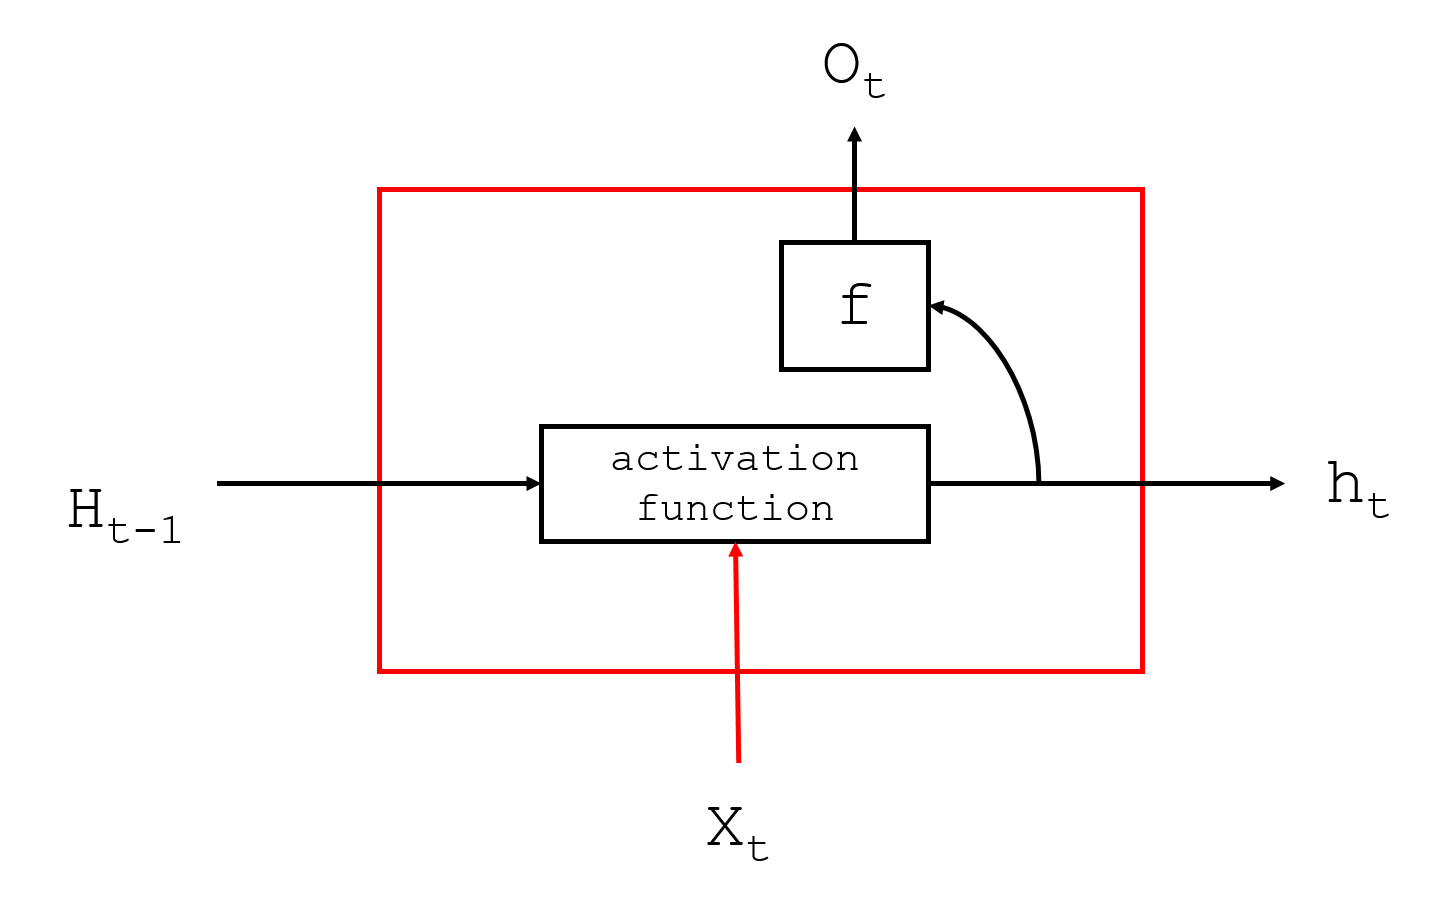
\includegraphics[width=0.80\linewidth]{images/nodes_rnn}
	\caption{1 buah \textit{timestep} dalam RNNs}
	\label{fig:nodes_rnn}
\end{figure}

\subsection{Long Short Term Memories (LSTMs)}\label{subbab:lstm}
Pada penjelasan di atas, RNNs sederhana memiliki kelebihan mempertimbangkan konteks untuk mengolah \textit{input} menjadi \textit{output}. Sayangnya, \textit{range} konteks yang dapat digunakan dalam satu blok terbatas \citep{graves2012neural}. Efek dari keterbatasan ini yaitu informasi pada suatu blok akan hilang atau terganggu dalam perjalanan \textit{timestep} sehingga \textit{output} yang dihasilkan tidak sesuai harapan. Oleh karena itu RNNs sederhana tidak dapat menangani permasalahan dependensi jangka panjang. Permasalahan ini disebut dengan \textit{vanishing gradient problem} (\cite{hochreiter1991untersuchungen}; \cite{hochreiter2001gradient}; \cite{bengio1994learning}). Banyak upaya untuk mengatasi masalah ini, seperti dengan menggunakan \textit{simulated annealing} dan \textit{discrete error propagation} \citep{bengio1994learning}, menggunakan \textit{time delays} (\cite{lang1990time}; \cite{bakker2001reinforcement}) atau \textit{time constant} \citep{ieee1997advances}, dan \textit{hierarchical sequence compression} \citep{schmidhuber2007training}. Namun sejauh ini solusi yang paling bagus yaitu dengan arsitektur \textit{Long Short Term Memory} (LSTM) \citep{hochreiter1997long}.

\begin{figure}
	\centering
	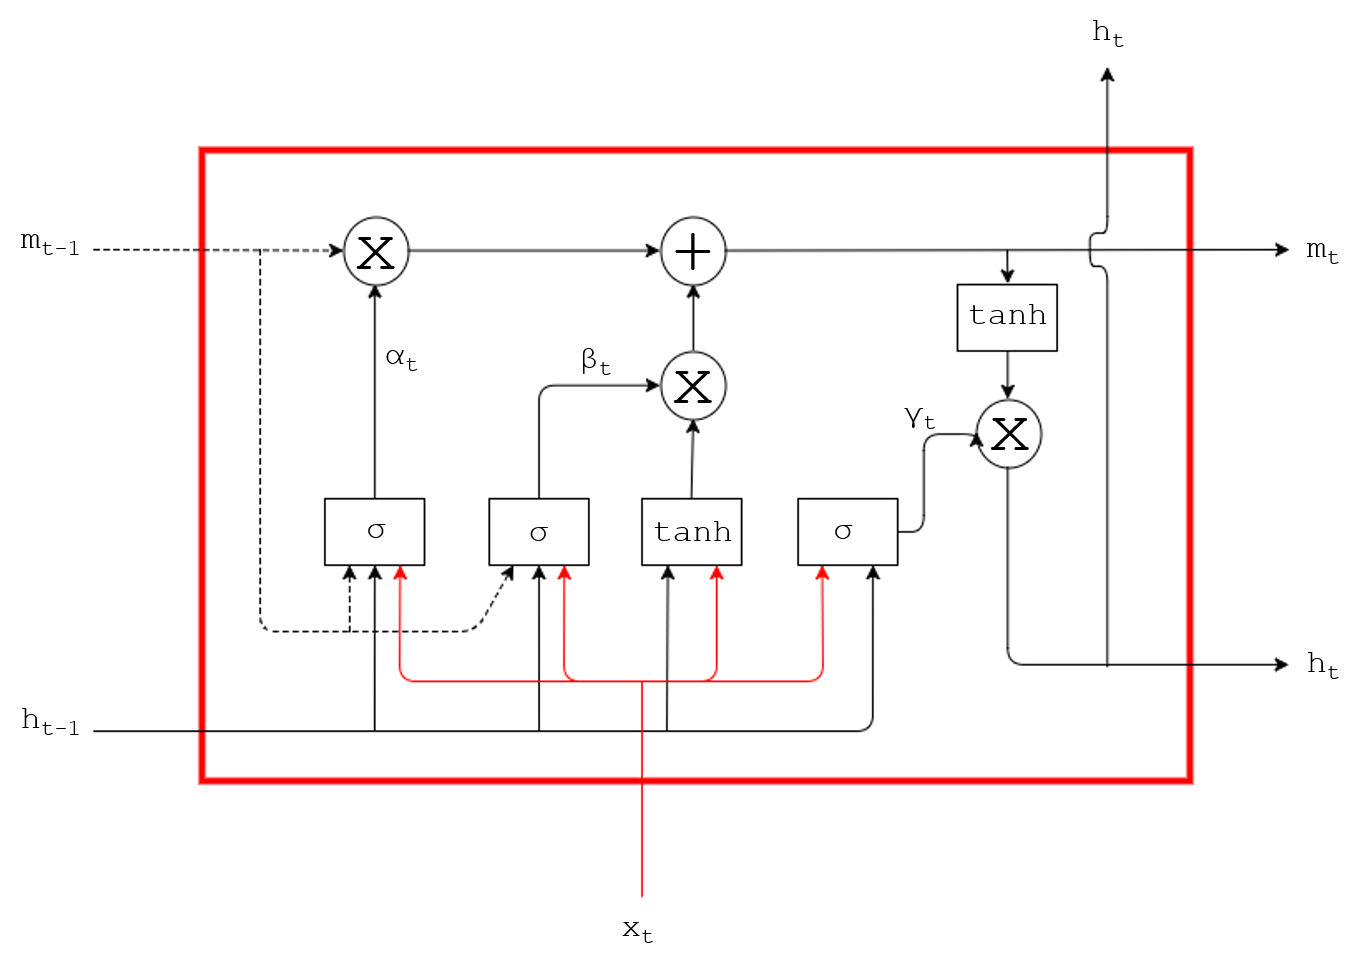
\includegraphics[width=1.0\linewidth]{images/lstm}
	\caption{1 buah blok memori dalam LSTM}
	\label{fig:lstm}
\end{figure}

LSTMs diperkenalkan oleh \cite{hochreiter1997long} dan saat ini banyak digunakan dalam berbagai \textit{task}. Gambar \ref{fig:lstm} merupakan ilustrasi satu buah blok memori di dalam LSTMs. Pada dasarnya, arsitektur LSTMs mirip dengan RNNs sederhana, namun unit \textit{nonlinear} pada \textit{hidden layer} di dalam RNNs sederhana diganti menjadi blok memori. Sebuah blok memori memiliki gerbang \textit{multiplicative} yang berfungsi untuk menyimpan dan mengakses informasi dari blok sebelumnya namun dengan batasan yang jauh lebih besar dibanding RNNs, sehingga mampu menghindari \textit{vanishing gradient problem}. Apabila \textit{input gate} selalu tertutup, maka memori tidak akan perah ditimpa sehingga isi memori tidak berubah.

Pada gambar \ref{fig:lstm}, kita dapat melihat bahwa 1 blok memori pada LSTMs tersebut memiliki 3 buah gerbang, yang berfungsi untuk sebagai pengatur suatu informasi apakah ditambahkan, dipertahankan atau dihapus di dalam sebuah sel. Masing-masing gerbang terdiri dari komponen \textit{sigmoid layer} dan komponen untuk melakukan operasi penjumlahan atau perkalian untuk masing-masing \textit{element-wise}. \textit{Sigmoid layer} tersebut memiliki nilai antara nol sampai dengan satu, yang mendeskripsikan perilaku gerbang dalam menerima \textit{input}. Semakin kecil nilai dari layer tersebut maka semakin kecil pula informasi masuk ke gerbang terkait dan sebaliknya. 

\begin{enumerate}
	\item \textit{Forget Gate}\\
	Gerbang ini memiliki fungsi untuk menentukan informasi yang akan disimpan di dalam memori dengan formula berikut
	\begin{equation}\label{eq:forget_lstm}
	\alpha_{t}=\sigma(W_{x\alpha}\cdot x_{t}+W_{h\alpha}\cdot~h_{t-1}+W_{m\alpha}\cdot~m_{t-1})
	\end{equation}
	
	\item \textit{Input Gate}\\
	Gerbang ini berfungsi untuk menentukan apakah informasi baru $ x(t) $ akan disimpan dalam \textit{cell state} atau tidak. 
	\begin{equation}\label{eq:input_lstm}
	\beta_{t}=\sigma(W_{x\beta}\cdot x_{t}+W_{h\beta}\cdot~h_{t-1}+W_{m\beta}\cdot~m_{t-1})
	\end{equation}
	
	\item \textit{Output Gate}\\
	Gerbang ini berfungsi untuk menendukan \textit{output} dari sebuah \textit{timestep} berdasarkan \textit{cell state} saat ini.
	\begin{equation}\label{eq:output_lstm}
	\gamma_{t}=\sigma(W_{x\gamma}\cdot x_{t}+W_{h\gamma}\cdot~h_{t-1}+W_{m\gamma}\cdot~m_{t-1})
	\end{equation}
	
\end{enumerate}

Dalam setiap \textit{timestep} $ t $, berikut merupakan formula untuk menghitung $ m(t) $ dan $ h(t) $:
\begin{equation}\label{eq:mt}
m_{t}=\alpha_{t} (\times) m_{t-1} + \beta_{t} (\times) f(x_{t},{t-1})
\end{equation}
\begin{equation}\label{eq:ht}
h_{t}=\gamma_{t} (\times) tanh(m_{t})
\end{equation}
dimana
\begin{equation}\label{eq:hf}
f(x_{t},{t-1})=tanh(W_{xm} \cdot x_{t} + W_{hm} \cdot h_{t-1})
\end{equation}

Notasi $ (\times) $ merupakan operasi perkalian untuk setiap pasang elemen, dan $ (+) $ merupakan operasi penjumlahan setiap pasang elemen.

\subsection{Penerapan RNNs untuk MER}
Terdapat beberapa penelitian terkait \mer~yang dikembangkan menggunakan RNNs, seperti \textit{drug entity recognition} \citep{mujiono2016new}, \textit{medical event detection on EHR} \citep{jagannatha2016bidirectional}, \textit{biomedical entity recognition} \citep{limsopatham2016learning}, dan \textit{Named Entity Recognition in Swedish Health Records} \citep{almgren2016named}. Penelitian \textit{drug entity recognition} oleh \cite{mujiono2016new} sudah dijelaskan pada subbab \ref{aboutmer}.

Dalam penelitiannya, \cite{jagannatha2016bidirectional} menggunakan LSTMs untuk memprediksi label entitasnya. Penelitian tersebut bertujuan untuk mendeteksi kejadian medis pada \textit{Electronic Health Records} seperti \textit{medication, diagnosis (Indication), adverse drug events (ADEs) severity, other SSD, frequency, drugname} dan \textit{duration}. Sebagai pembanding, penulis tersebut juga mengimplementasikan CRF dan GRU. Ada beberapa kesulitan yang dihadapi dalam mengolah EHR tersebut, yaitu EHR lebih \textit{noisy} dibandingkan dengan teks biasa, banyak kalimat yang tidak komplet dan penggunaan frasa. Hasil dari penelitian tersebut menunjukkan bahwa semua model RNNs (LSTMs dan GRU) memiliki akurasi yang lebih baik daripada CRF. Apabila dibandingkan dengan \textit{baseline} yang digunakan, GRU mampu meningkatkan \textit{recall} (0.8126), \textit{precision} (0.7938) dan \textit{F-score} (0.8031) sebesar 19\%, 2\% dan 11\% dari \textit{baseline}.

\cite{limsopatham2016learning} menggunakan \textit{Bidirectional-LSTMs} untuk mengidentifikasi kalimat dengan menggunakan karakter dan kata yang diubah menjadi vektor menggunakan \textit{word embedding}. Untuk setiap kalimatnya, peneliti tersebut mengusulkan adanya \textit{ortographic feature} supaya modelnya dapat mempelajari fitur tersebut secara eksplisit. Evaluasi yang digunakan menggunakan tiga buah koleksi \textit{biomedical test}, yaitu \textit{Gene Mention task corpus}, \textit{BioNLP 2009} dan \textit{NCBI disease corpus}, dengan perhitungan \textit{F1-score}. ada empat \textit{baseline} yang digunakan sebagai pembanding, yaitu \textit{feedforward}, \textit{bidirectional-LSTM}, \textit{CNN-Bidirectional-LSTM} yang hanya menggunakan karakter dan \textit{CNN-Bidirectional LSTM}. Hasil yang didapatkan mengatakan bahwa penggunaan \textit{Bidirectional-LSTM} yang dikombinasikan dengan CNN dengan diberikan \textit{word embedding} dan \textit{orthographic} merupakan model yang paling bagus. Penulis tersebut juga menyimpulkan bahwa penggunaan fitur \textit{hand-crafted} tersebut mampu memberikan akurasi yang lebih tinggi.

\cite{almgren2016named} menggunakan \textit{deep bidirectional LSTM} dalam mengembangkan NER di bidang medis. Entitas yang akan diidentifikasi adalah \textit{disorders and findings}, \textit{pharmaceutical drugs}, \textit{body structure} dan \textit{non-entity term}. Model menggunakan teks medis berbahasa Swedia sebagai \textit{dataset}, di-\textit{train} dengan menggunakan \textit{end-to-end backpropagation} dan Adam \textit{optimizer}, dan \textit{input} yang diberikan berbentuk urutan karakter. Hasil yang didapatkan adalah Char-BiLSTM pada Stockholm EPR corpus mendapatkan \textit{precision} 0.67, \textit{recall} 0.12 dan \textit{f-measure} 0.20 meningkat 60\% dibandingkan dengan \textit{baseline}.

\section{Word Embedding}
Pada umumnya, pendekatan yang digunakan untuk merepresentasikan sebuah kata sebagai \textit{input} model adalah dengan menggunakan \textit{one-hot-vetor} \citep{turian2010word}. Panjang dari sebuah vektor kata ini bergantung dari banyaknya kata unik di dalam sebuah korpus. Ada beberapa cara untuk mengubahnya menjadi \textit{one-hot-vector}, seperti mengumpulkan semua kata unik kemudian mngurutkannya secara alfabetis. Vektor \textit{one-hot} tersebut bernilai 1 pada indeks kata yang bersesuaian. Misalnya kata "obat" berada di indeks ke 25 pada kumpulan kata unik, maka representasi vektornya elemen ke 21 di vektor "obat" adalah 1 sedangkan yang lainnya 0.

Dari ilustrasi singkat tersebut, representasi \textit{one-hot-vector} memiliki kelemahan yaitu besar vektor yang tergantung jumlah kata unik di dalam korpus. Selain itu, jika terdapat sebuah kata yang muncul di korpus namun tidak muncul di \textit{training} ataupun \textit{testing data}, kata tersebut tidak dapat diproses. Selain itu, sangat susah untuk mencari hubungan baik sintak maupun semantik dari representasi kata ini, karena antar kata hanya dibedakan indeks yang berisi angka 1 saja.

Dari kelemahan di atas, terdapat sebuah representasi vektor lain dari kata yang lebih baik, yaitu dengan menggunakan \textit{word embedding}. \textit{Word embedding} adalah salah satu jenis dari representasi kata yang memiliki kelebihan yaitu padat, berdimensi rendah, dan memiliki nilai yang real. \textit{Word embedding} memetakan kata dengan vektor berisi bilangan \textit{real}, misalkan W("obat") = [0.4, -0.9, 0.1, ...., 0.9], dimana W adalah fungsi yang memetakan suatu kata menuju representasi vektor dan W("obat") merupakan \textit{word embedding} dari kata "obat". \textit{Word embedding} dapat meningkatkan performa dari \textit{tasks} dalam NLP dengan cara mengelompokkan kata-kata yang mirip, karena kata yang mirip memiliki vektor yang mirip pula. Ada beberapa metode \textit{word embedding} yang banyak digunakan dalam beberapa \textit{task} di NLP, seperti Glove \citep{pennington2014glove} dan Word2Vec \citep{mikolov2014word2vec}. Pada pembahasan ini, \saya~hanya menuliskan mengenai Word2Vec.

Word2Vec merupakan model linguistik yang dikembangkan oleh \cite{mikolov2014word2vec} dan berdasarkan pada \textit{neural networks}. Word2Vec mempelajari \textit{embedding} dari setiap kata untuk dipetakan ke masing-masing vektor yang berdimensi rendah dari sifat distribusinya pada korpus yang diberikan. Dari situ, Word2Vec mampu mengelompokkan kata berdasarkan kemiripannya di dalam \textit{vector space}.

\begin{figure}
	\centering
	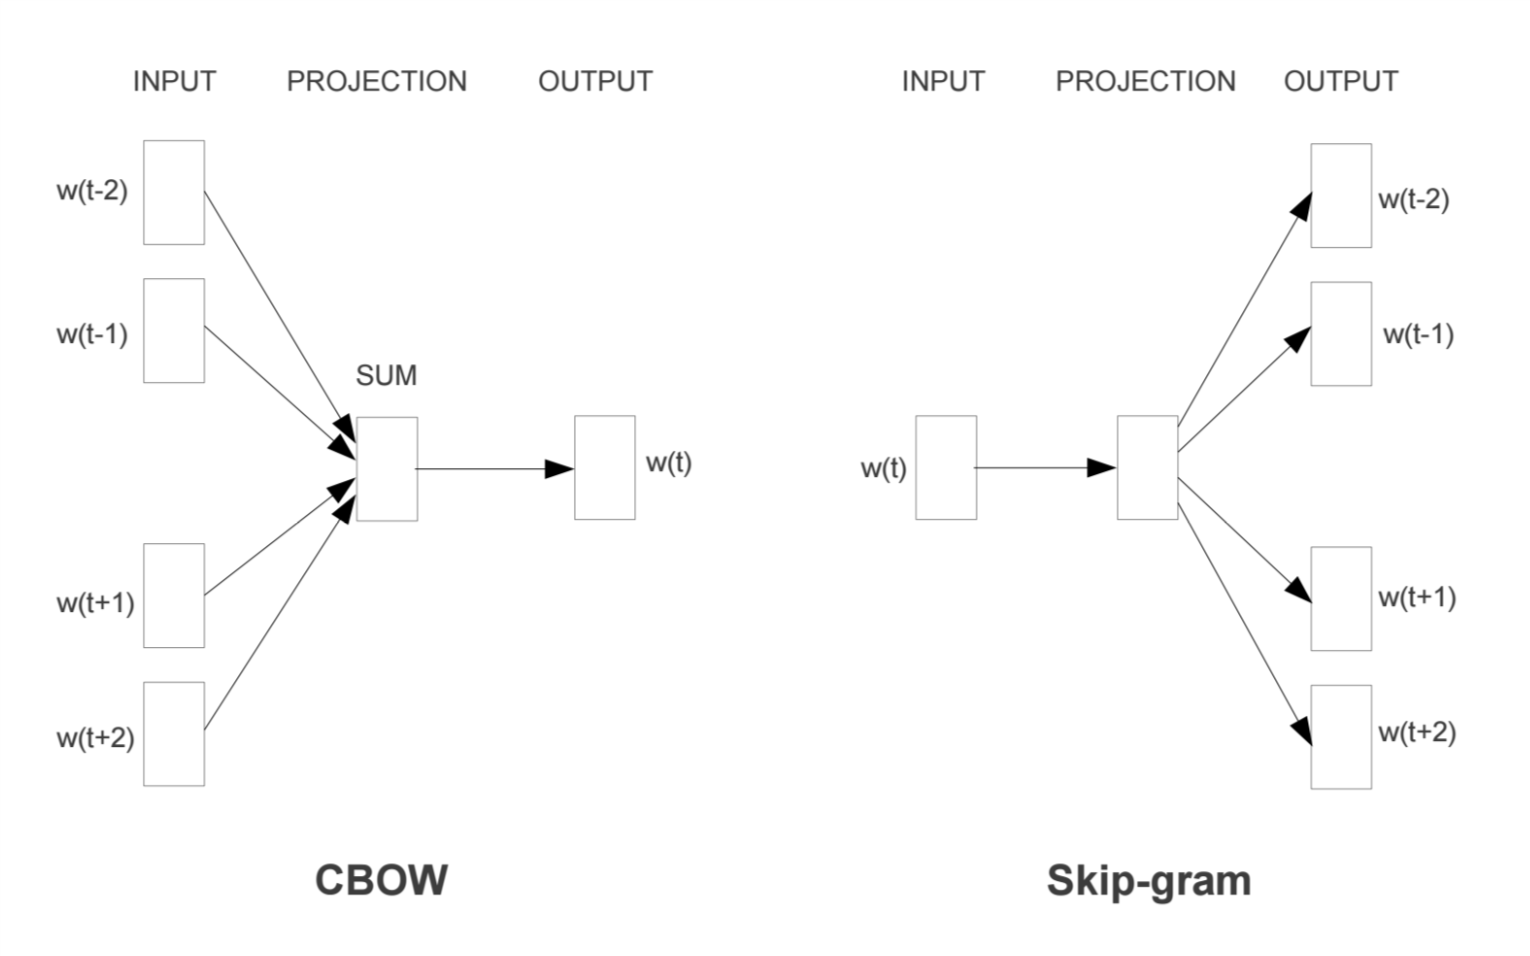
\includegraphics[width=0.85\linewidth]{images/word2vec}
	\caption{Arsitektur Word2Vec}
	\label{fig:word2vec}
\end{figure}

Ada dua arsitektur Word2Vec yang dikembangkan oleh \cite{mikolov2014word2vec}, yaitu arsitektur \textit{skip-gram} dan arsitektur \textit{continuous bag-of-words} (CBOW). Dari gambar \ref{fig:word2vec}, dapat dilihat bahwa arsitektur CBOW memprediksi masing-masing kata berdasarkan kata di sekelilingnya. \textit{Input layer} dalam arsitektur ini direpresentasikan dengan \textit{bag-of-words}. CBOW sendiri dapat mempelajari data dengan ukuran yang sangat besar yang tidak dapat dilakukan oleh model \textit{neural network} yang lain. Sedangkan arsitektur \textit{skip-gram} memprediksi kata-kata di sekeliling dan konteksnya berdasarkan sebuah kata yang diberikan (gambar \ref{fig:word2vec}). \textit{Skip-gram} mampu menangkap \textit{co-occurance} rata-rata dari dua buah kata di dalam \textit{training set}.
%-----------------------------------------------------------------------------%
% Cerita umum Word Embedding terlepas dari, kenapa bukan %
% Salah satunya adalah word2vc%
% CBOW vs Skip %
